\documentclass[12pt]{article}
\usepackage[paper=letterpaper,margin=2cm]{geometry}
\usepackage{amsmath,amssymb,amsfonts}
\usepackage{newtxtext,newtxmath}
\usepackage{enumitem}
\usepackage{titling}
\usepackage{subfig,graphicx}
\usepackage[colorlinks=true]{hyperref}
\usepackage{multirow}
\usepackage{listings}
\usepackage{xcolor}
\usepackage{float}

\definecolor{codegreen}{rgb}{0,0.6,0}
\definecolor{codegray}{rgb}{0.5,0.5,0.5}
\definecolor{codepurple}{rgb}{0.58,0,0.82}
\definecolor{backcolour}{rgb}{0.95,0.95,0.92}

\lstdefinestyle{mystyle}{
    commentstyle=\color{codegreen},
    keywordstyle=\color{magenta},
    numberstyle=\tiny\color{codegray},
    stringstyle=\color{codepurple},
    basicstyle=\ttfamily\footnotesize,
    breakatwhitespace=false,
    breaklines=true,
    captionpos=b,
    keepspaces=true,
    numbers=left,
    numbersep=5pt,
    showspaces=false,
    showstringspaces=false,
    showtabs=false,
    tabsize=2
}
\lstset{style=mystyle}

\begin{document}

\begin{center}
\large{Aprendizagem 2023}\\
Homework I -- Group 28\\
\vskip 0.3cm
Gonçalo Bárias (ist1103124) \& Raquel Braunschweig (ist1102624)\vskip 1cm

\large{\textbf{Part I}: Pen and Paper}\normalsize
\end{center}

\noindent Consider the partially learnt decision tree from the dataset $D$. $D$ is described by four input variables –
one numeric with values in $[0,1]$ and 3 categorical – and a target variable with three classes.

\begin{figure}[H]
    \centering
    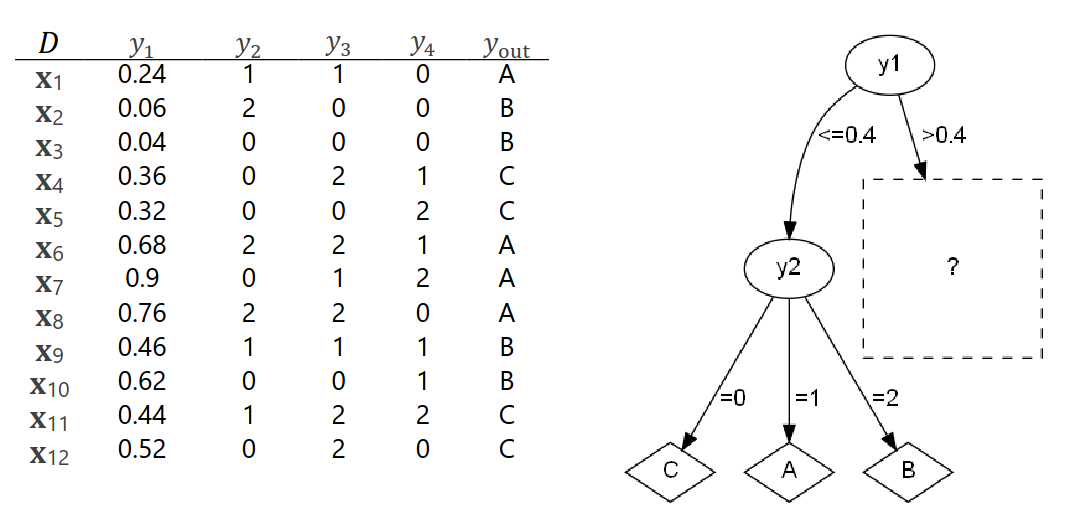
\includegraphics[width=15cm]{./assets/partial_tree_dataset_d}
    \label{fig:PartI-partial-decision-tree-dataset-d}
\end{figure}

\begin{enumerate}[leftmargin=\labelsep]
    \item \textbf{Complete the given decision tree using Information gain with Shannon entropy ($log_2$).
    Consider that: i) a minimum of 4 observations is required to split an internal node, and
    ii) decisions by ascending alphabetic order should be placed in case of ties.}

    \vskip 0.3cm
    The entropy of \(y_{out}\) is given by:

    \begin{equation}
        \begin{split}
            E(y_{out} |y_1 > 0.4) =
            & - P(y_{out} = \text{A}, y_1 > 0.4) \log_2 \left(P(y_{out} = \text{A}, y_1 > 0.4)\right) \\
            & - P(y_{out} = \text{B}, y_1 > 0.4) \log_2 \left(P(y_{out} = \text{B}, y_1 > 0.4)\right)      \\
            & - P(y_{out} = \text{C}, y_1 > 0.4) \log_2 \left(P(y_{out} = \text{C}, y_1 > 0.4)\right)      \\
        \end{split}
    \end{equation}

    We can calculate $E(y_{out})$:

    \[
        \begin{aligned}
            E(y_{out} |y_1 > 0.4) & = - \left(\frac{3}{7} \log_2\left(\frac{3}{7}\right) + \frac{2}{7} \log_2\left(\frac{2}{7}\right)
                            + \frac{2}{7} \log_2\left(\frac{2}{7}\right)\right) \approx 1.5567
        \end{aligned}
    \]

    The next step is calculating $E(y_{out} | y_1 > 0.4 , y_x)$, in which x will take the values of 2, 3 or 4:

    \begin{equation}\label{exI1-e-yout-y2}
        \begin{split}
            E(y_{out} |y_1 > 0.4 , y_x) =
            & - P(y_x = 0) E(y_{out} | y_1 > 0.4 , y_x = 0) \\
            & - P(y_x = 1) E(y_{out} | y_1 > 0.4 , y_x = 1) \\
            & - p(y_x = 2) E(y_{out} | y_1 > 0.4 , y_x = 2)
        \end{split}
    \end{equation}

    And the information gain of variable $y_x$ is given by

    \begin{equation}\label{ex1-ig}
        IG(y_{out} |y_1 > 0.4, y_x) = E(y_{out} |y_1 > 0.4) - E(y_{out} |y_1 > 0.4, y_x)
    \end{equation}

    \textbf{Let's start with x = 2}:

    \[
        \begin{aligned}
            P(y_2 = 0, y_1 > 0.4)          & = \frac{3}{7}                                                                                       \\
            P(y_2 = 1, y_1 > 0.4)          & = \frac{2}{7}                                                                                       \\
            P(y_2 = 1, y_1 > 0.4)          & = \frac{2}{7}                                                                                       \\
            E(y_{out} | y_1 > 0.4 , y_2 = 0) & = - \left(\frac{1}{3} \log_2\left(\frac{1}{3}\right) + \frac{1}{3} \log_2\left(\frac{1}{3}\right)
                + \frac{1}{3} \log_2\left(\frac{1}{3}\right)\right) \approx 1.58493                                                              \\
            E(y_{out} | y_1 > 0.4 , y_2 = 1) & = - \left(\frac{0}{2} \log_2\left(\frac{0}{2}\right) + \frac{1}{2} \log_2\left(\frac{1}{2}\right)
                + \frac{1}{2} \log_2\left(\frac{1}{2}\right)\right) = 1                                                                          \\
            E(y_{out} | y_1 > 0.4 , y_2 = 2) & = - \left(\frac{2}{2} \log_2\left(\frac{2}{2}\right) + \frac{0}{2} \log_2\left(\frac{0}{2}\right)
                + \frac{0}{2} \log_2\left(\frac{0}{2}\right)\right) = 0
        \end{aligned}
    \]

    Therefore, replacing these values on equation \eqref{exI1-e-yout-y2}, gives us:

    \[
        \begin{aligned}
            E(y_{out} | y_1>0.4, y_2) & = \frac{3}{7} \times 1.58493 + \frac{2}{7} \times 1 + \frac{2}{7} \times 0 & \approx 0.965.
        \end{aligned}
    \]

    Finally, we can calculate the information gain, as per \eqref{ex1-ig},

    \[
        IG(y_{out} |y_1 > 0.4, y_{2}) = 1.5567 - 0.965 = 0.5917
    \]

    \textbf{Now, let's calculate for x = 3}:

    \[
        \begin{aligned}
            P(y_3 = 0, y_1 > 0.4)          & = \frac{1}{7}                                                                                       \\
            P(y_3 = 1, y_1 > 0.4)          & = \frac{2}{7}                                                                                       \\
            P(y_3 = 2, y_1 > 0.4)          & = \frac{4}{7}                                                                                       \\
            E(y_{out} | y_1 > 0.4 , y_3 = 0) & = - \left(\frac{0}{1} \log_2\left(\frac{0}{1}\right) + \frac{1}{1} \log_2\left(\frac{1}{1}\right)
                + \frac{0}{1} \log_2\left(\frac{0}{1}\right)\right) = 0                                                                          \\
            E(y_{out} | y_1 > 0.4 , y_3 = 1) & = - \left(\frac{1}{2} \log_2\left(\frac{1}{2}\right) + \frac{1}{2} \log_2\left(\frac{1}{2}\right)
                + \frac{0}{2} \log_2\left(\frac{0}{2}\right)\right) = 1                                                                          \\
            E(y_{out} | y_1 > 0.4 , y_3 = 2) & = - \left(\frac{2}{4} \log_2\left(\frac{2}{4}\right) + \frac{0}{4} \log_2\left(\frac{0}{4}\right)
                + \frac{2}{4} \log_2\left(\frac{2}{4}\right)\right) = 1
        \end{aligned}
    \]

    Therefore, replacing these values on equation \eqref{exI1-e-yout-y2}, gives us:

    \[
        \begin{aligned}
            E(y_{out} | y_1>0.4, y_3) & = \frac{1}{7} \times 0 + \frac{2}{7} \times 1 +  \frac{4}{7} \times 1 & \approx 0.8571.
        \end{aligned}
    \]

    Finally, we can calculate the information gain, as per \eqref{ex1-ig},

    \[
        IG(y_{out} | y_1 > 0.4, y_{3}) = 1.5567 - 0.8571 = \textbf{0.6996}
    \]

    \textbf{Finally, let's calculate for x = 4}:

    \[
        \begin{aligned}
            P(y_4 = 0, y_1 > 0.4)          & = \frac{2}{7}                                                                                       \\
            P(y_4 = 1, y_1 > 0.4)          & = \frac{3}{7}                                                                                       \\
            P(y_4 = 1, y_1 > 0.4)          & = \frac{2}{7}                                                                                       \\
            E(y_{out} | y_1 > 0.4 , y_4 = 0) & = - \left(\frac{1}{2} \log_2\left(\frac{1}{2}\right) + \frac{0}{2} \log_2\left(\frac{0}{2}\right)
                + \frac{1}{2} \log_2\left(\frac{1}{3}\right)\right) = 1                                                                          \\
            E(y_{out} | y_1 > 0.4 , y_4 = 1) & = - \left(\frac{1}{3} \log_2\left(\frac{1}{3}\right) + \frac{2}{3} \log_2\left(\frac{2}{3}\right)
                + \frac{0}{3} \log_2\left(\frac{0}{3}\right)\right) \approx 0.9183                                                               \\
            E(y_{out} | y_1 > 0.4 , y_4 = 2) & = - \left(\frac{1}{2} \log_2\left(\frac{1}{2}\right) + \frac{0}{2} \log_2\left(\frac{0}{2}\right)
                + \frac{1}{2} \log_2\left(\frac{1}{2}\right)\right) = 1
        \end{aligned}
    \]

    Therefore, replacing these values on equation \eqref{exI1-e-yout-y2}, gives us:

    \[
        \begin{aligned}
            E(y_{out} | y_1>0.4, y_4) & = \frac{2}{7} \times 1 + \frac{3}{7} \times 0.9183 +  \frac{2}{7} \times 1 \approx 0.965.
        \end{aligned}
    \]

    Finally, we can calculate the information gain, as per \eqref{ex1-ig},

    \[
        IG(y_{out} | y_1 > 0.4, y_{4}) = 1.5567 - 0.965 = 0.5917
    \]

    \textbf{Upon computing the information gains for each attribute,} it is evident that $y_3$ yields the highest value of 0.6996. Consequently,
        it is selected as the next node, and since there are at least 4 observations with $y_1 > 0.4$, we split the new node.

    If we fix $y_1 > 0.4$ with $y_3 = 0$ or $y_3 = 1$, we get 1 and 2 observations, respectively. This means we get two new leafs for those branches, with
    the $y_3 = 0$ leaf equal to class \text{B} and the $y_3 = 1$ leaf equal to \text{A}, because those are the classes that have the highest frequency for
    their respective conditions on the dataset. For the $y_3 = 1$ leaf there is a tie, which we just use the ascending alphabetic order to get the class.
    For the $y_3 = 2$ branch with the $y_1 > 0.4$ condition, we get exactly 4 observations, and so there is a split.

    \textbf{Below} we do the required calculations to finish the decision tree:

    \[
        \begin{aligned}
            E(y_{out} | y_1 > 0.4 , y_3 = 2 , y_2 = 0) & = - \left(\frac{0}{1} \log_2\left(\frac{0}{1}\right) + \frac{0}{1} \log_2\left(\frac{0}{1}\right)
                + \frac{1}{1} \log_2\left(\frac{1}{1}\right)\right) = 0                                                                          \\
            E(y_{out} | y_1 > 0.4 , y_3 = 2 , y_2 = 1) & = - \left(\frac{0}{1} \log_2\left(\frac{0}{1}\right) + \frac{0}{1} \log_2\left(\frac{0}{1}\right)
                + \frac{1}{1} \log_2\left(\frac{1}{1}\right)\right) = 0                                                                          \\
            E(y_{out} | y_1 > 0.4 , y_3 = 2 , y_2 = 2) & = - \left(\frac{2}{2} \log_2\left(\frac{2}{2}\right) + \frac{0}{2} \log_2\left(\frac{0}{2}\right)
                + \frac{0}{2} \log_2\left(\frac{0}{2}\right)\right) = 0                                                                          \\
            E(y_{out} | y_1 > 0.4 , y_3 = 2 , y_4 = 0) & = - \left(\frac{1}{2} \log_2\left(\frac{1}{2}\right) + \frac{0}{2} \log_2\left(\frac{0}{2}\right)
                + \frac{1}{2} \log_2\left(\frac{1}{2}\right)\right) = 1                                                                          \\
            E(y_{out} | y_1 > 0.4 , y_3 = 2 , y_4 = 1) & = - \left(\frac{1}{1} \log_2\left(\frac{1}{1}\right) + \frac{0}{1} \log_2\left(\frac{0}{1}\right)
                + \frac{0}{1} \log_2\left(\frac{0}{1}\right)\right) = 0                                                                          \\
            E(y_{out} | y_1 > 0.4 , y_3 = 2 , y_4 = 2) & = - \left(\frac{0}{1} \log_2\left(\frac{0}{1}\right) + \frac{0}{1} \log_2\left(\frac{0}{1}\right)
                + \frac{1}{1} \log_2\left(\frac{1}{1}\right)\right) = 0
        \end{aligned}
    \]

    From other calculations above, we know that:

    \[
        E(y_{out} | y_1 > 0.4 , y_3 = 2) = 1
    \]

    Therefore, replacing the above values on equation \eqref{exI1-e-yout-y2}, gives us:

    \[
        \begin{aligned}
            E(y_{out} | y_1>0.4, y_3 = 2, y_2) & = \frac{1}{4} \times 0 + \frac{1}{4} \times 0 + \frac{2}{4} \times 0 = 0 \\
            E(y_{out} | y_1>0.4, y_3 = 2, y_4) & = \frac{2}{4} \times 1 + \frac{1}{4} \times 0 + \frac{1}{4} \times 0 = 0.5
        \end{aligned}
    \]

    Finally, we can calculate the information gain, as per \eqref{ex1-ig},

    \[
        \begin{aligned}
            IG(y_{out} |y_1 > 0.4, y_3 = 2, y_{2}) & = 1 - 0 = \textbf{1} \\
            IG(y_{out} |y_1 > 0.4, y_3 = 2, y_{4}) & = 1 - 0.5 = 0.5
        \end{aligned}
    \]

    \textbf{After the computation}, it is evident that $y_2$ yields the highest value of 1, and so it is chosen. With the conditions of $y_1 > 0.4$ and $y_3 = 2$, we
    can check that the conditions $y_2 = 0$, $y_2 = 1$ and $y_2 = 2$ all have less than 4 observations each. Therefore, we take the class with the highest frequency
    for each respective conditions on the dataset. \textbf{Finally}, we can construct the following decision tree:

    \begin{figure}[H]
        \centering
        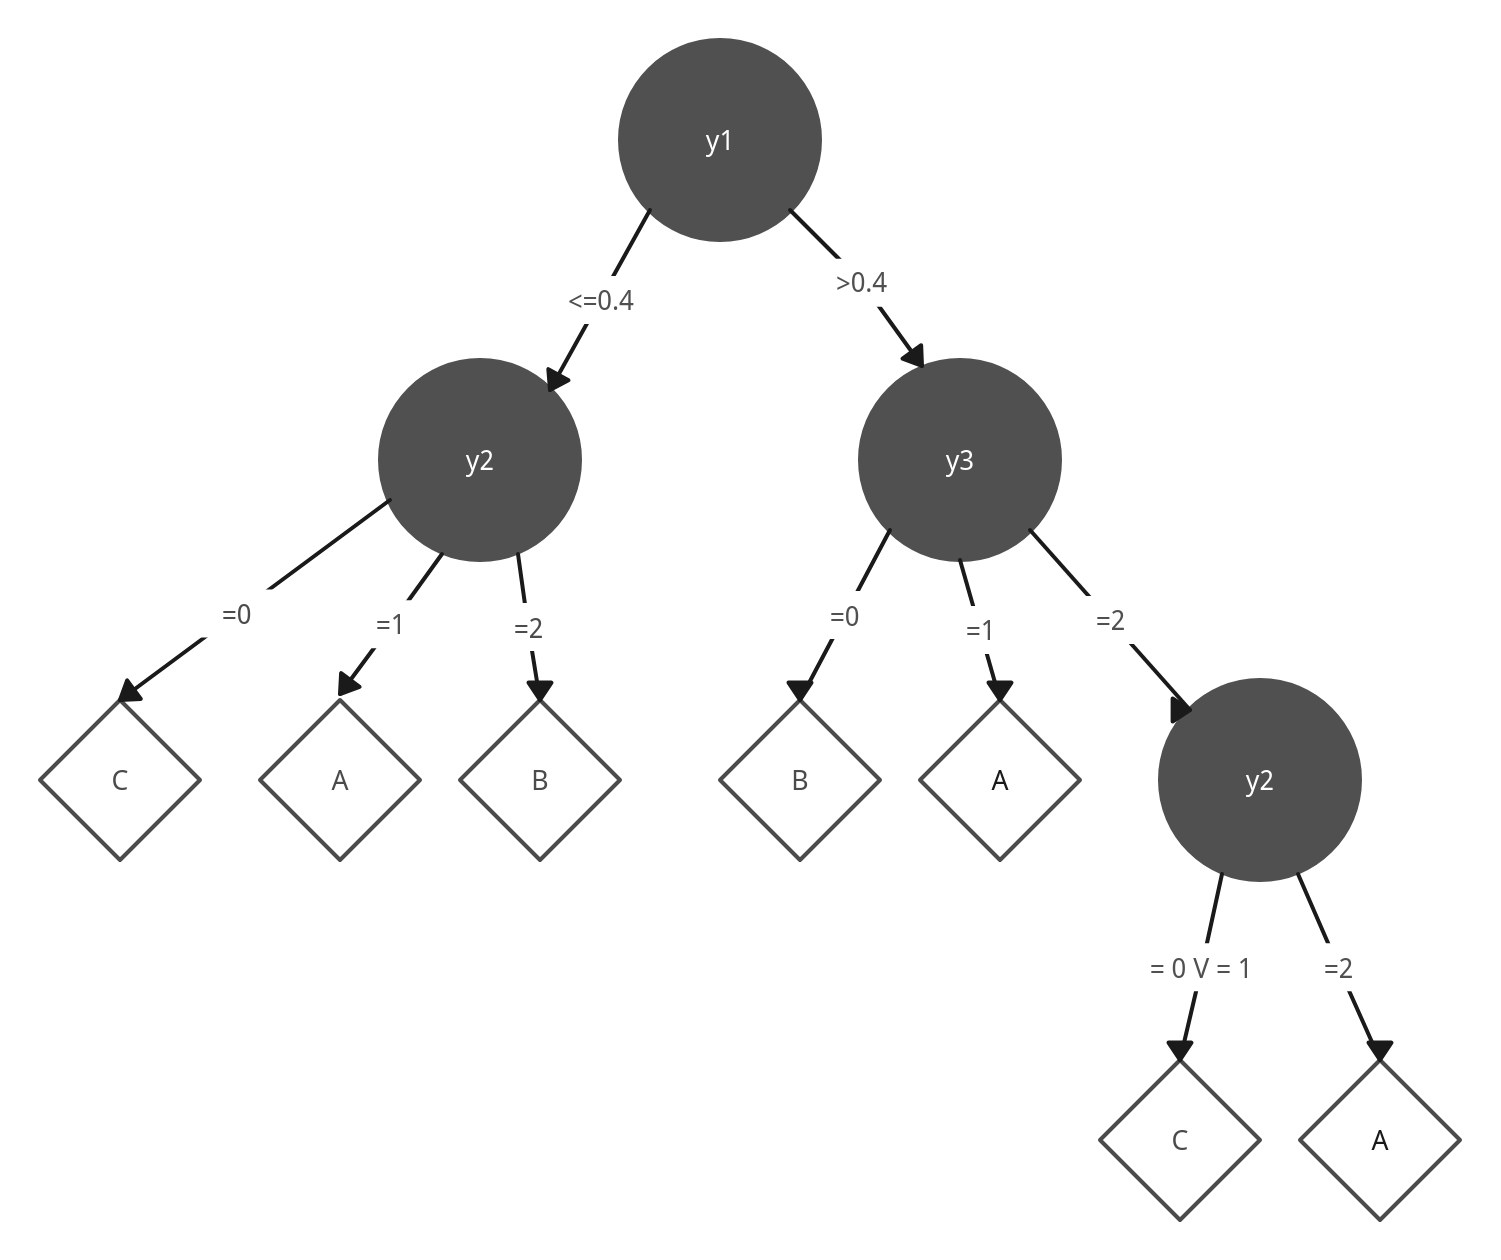
\includegraphics[width=12cm]{./assets/decision_tree_ex1_PartI.png}
        \caption{Decision Tree for exercise I.1}
        \label{fig:decision_tree}
    \end{figure}

    \item \textbf{Draw the training confusion matrix for the learnt decision tree.}

    \vskip 0.3cm
    Following the learnt decision tree above, we can predict the values for each observation.
    For each observation, we look at the value for the first variable ($y_1$) and follow the branch that corresponds with its value.
    From the node we arrive at, we do the same thing for the next variable, and we keep doing this until we reach a leaf.
    The class present in this leaf will be the predicted value, while the real value is the value of $y_{out}$ for that observation.
    Below we present the real values along with the predicted ones:

    \begin{center}
        \begin{tabular}{cccccccccccccc}
            \multicolumn{2}{c}{}           & $x_1$ & $x_2$ & $x_3$ & $x_4$ & $x_5$ & $x_6$ & $x_7$ & $x_8$ & $x_9$ & $x_{10}$ & $x_{11}$ & $x_{12}$ \\
            \multirow{1}{*}{real}      & = & [A   & B   & B   & C   & C   & A   & A   & A   & B   & B   & C   & C]                                  \\
            \multirow{1}{*}{predicted} & = & [A   & B   & C   & C   & C   & A   & A   & A   & A   & B   & C   & C]
        \end{tabular}
    \end{center}

    \textbf{Finally}, we can show the count of each pair of real and predicted values in a confusion matrix (e.g. 4 pairs of AA from observations $x_1$, $x_6$, $x_7$ and $x_8$):

    \vspace{0.5em}
    \begin{center}
        \begin{tabular}{|c|c|c|c|c|c|}
            \cline{3-5}
            \multicolumn{2}{c}{}                & \multicolumn{3}{|c|}{\textbf{Real}} & \multicolumn{1}{c}{}  \\
            \cline{3-5}
            \multicolumn{2}{c|}{}               & \textbf{A} & \textbf{B} & \textbf{C} & \multicolumn{1}{c}{} \\
            \hline
                                                & \textbf{A} & 4 & 1 & 0 & 5                                  \\
            \cline{2-6}
            \multirow{1}{*}{\textbf{Predicted}} & \textbf{B} & 0 & 2 & 0 & 2                                  \\
            \cline{2-6}
                                                & \textbf{C} & 0 & 1 & 4 & 5                                  \\
            \hline
            \multicolumn{2}{c|}{}               & 4 & 4 & 4 & 12                                              \\
            \cline{3-6}
        \end{tabular}
    \end{center}

    \item \textbf{Identify which class has the lowest training F1 score.}

    \vskip 0.3cm

    \(F1_{score}\) is given by the following equation:

    \begin{equation}\label{ex3-f1}
        F1_{score} = 2 \cdot \frac{{\text{Precision} \cdot \text{Recall}}}{{\text{Precision} + \text{Recall}}}
    \end{equation}

    And precision and recall are given by:

    \begin{equation}\label{e3-p}
        \text{Precision} = \frac{\text{True Positives}}{{\text{True Positives} + \text{False Positives}}}
    \end{equation}

    \begin{equation}\label{e3-r}
        \text{Recall} = \frac{\text{True Positives}}{{\text{True Positives} + \text{False Negatives}}}
    \end{equation}

    Therefore, \textbf{let's start by calculating the precision for A, B and C} by replacing the values on \eqref{e3-p}:

    \[
        \begin{aligned}
            Precision_A = \frac{4}{4+1} = \frac{4}{5}
        \end{aligned}
    \]

    \[
        \begin{aligned}
            Precision_B = \frac{2}{2+0} = 1
        \end{aligned}
    \]

    \[
        \begin{aligned}
            Precision_C = \frac{4}{4+1} = \frac{4}{5}
        \end{aligned}
    \]


    \textbf{Now, it's time to calculate the recalls for A, B and C}, using the equation on \eqref{e3-r}:

    \[
        \begin{aligned}
            Recall_A = \frac{4}{4+0} = 1
        \end{aligned}
    \]

    \[
        \begin{aligned}
            Recall_B = \frac{2}{2+2} = \frac{1}{2}
        \end{aligned}
    \]

    \[
        \begin{aligned}
            Recall_C = \frac{4}{4+0} = 1
        \end{aligned}
    \]

    \textbf{Finally, let's calculate the $F1_{score}$}, using the equation \eqref{ex3-f1}:

    \[
        \begin{aligned}
            F1_{score} A = 2 \cdot \frac{{ \frac{4}{5} \cdot 1 }}{{ \frac{4}{5} + 1 }} \approx 0.8889
        \end{aligned}
    \]

    \[
        \begin{aligned}
            F1_{score} B = 2 \cdot \frac{{ 1 \cdot \frac{1}{2} }}{{ 1 + \frac{1}{2} }} \approx 0.6667
        \end{aligned}
    \]

    \[
        \begin{aligned}
            F1_{score} C = 2 \cdot \frac{{ \frac{4}{5} \cdot 1 }}{{ \frac{4}{5} + 1 }} \approx 0,8889
        \end{aligned}
    \]

    \textbf{The class with the lowest training F1 score is B}, with a score of 0.6667.

    \item \textbf{Considering $y_2$ to be ordinal, assess if $y_1$ and $y_2$ are correlated using the Spearman coefficient.}

    \vskip 0.3cm

    To calculate the Spearman coefficient when there's rank, we have to use the following equation:

    \begin{equation}\label{ex4-sp}
        \begin{split}
            \text{Spearman}(y_x, y_y) = \text{Pearson}(y_x', y_y') = \frac{\text{cov}(y_x', y_y')}{\sigma_{y_x'} \sigma_{y_y'}}
            = \frac{\sum_{i=1}^{n} (y_{x_i}' - \bar{y_x'})(y_{y_i}' - \bar{y_y'})}{\sqrt{\sum_{i=1}^{n} (y_{x_i}' - \bar{y_x'})^2}\sqrt{\sum_{i=1}^{n} (y_{y_i}' - \bar{y_y'})^2}}
        \end{split}
    \end{equation}

    Firstly, \textbf{let's order $y_1$ and $y_2$} so we can calulate the ranks and $y'_1$ and $y'_2$:

    \begin{align*}
        ordered\_y_{1} & = [0.04, 0.06, 0.24, 0.32, 0.36, 0.44, 0.46, 0.52, 0.62, 0.68, 0.76, 0.9]\\
        ranks\_y_{1}   & = [1,2,3,4,5,6,7,8,9,10,11,12]\\
        y'_{1}         & = [3,2,1,5,4,10,12,11,7,9,6,8]\\
        ordered\_y_{2} & = [0,0,0,0,0,0,1,1,1,2,2,2]\\
        ranks\_y_{2}   & = [3.5, 3.5, 3.5, 3.5, 3.5, 3.5, 8, 8, 8, 11, 11, 11]\\
        y'_{2}         & = [8, 11, 3.5, 3.5, 3.5, 11, 3.5, 11, 8, 3.5, 8, 3.5]
    \end{align*}

    Now, we have all we need to calculate \textbf{the Spearman coefficient} using the expression at \eqref{ex4-sp}. Here is the result:

    \[
        Spearman(y_{1}, y_{2}) = Pearson(y_{1}', y_{2}') \approx 0.07966
    \]

    Since the rank correlation (under Spearman coefficient) obtained a value relatively close to 0, we can conclude that the variables $y_1$ and $y_2$ are almost non correlated.

    \item \textbf{Draw the class-conditional relative histograms of $y_1$ using 5 equally spaced bins in $[0,1]$.
    Find the root split using the discriminant rules from these empirical distributions.}

    \vskip 0.3cm
    The following histograms were created by observing the values of $y_1$ and fixing the class in $y_{out}$. Since there are three classes $A$, $B$ and $C$,
    we get three histograms. In each histogram we have 5 equally spaced bins in $[0,1]$, meaning that each bin has a length of $0.2$. For each class, when a value
    of $y_1$ falls into a bin, we increase the value of that bin by one.

    \begin{figure}[H]
        \centering
        \subfloat[]{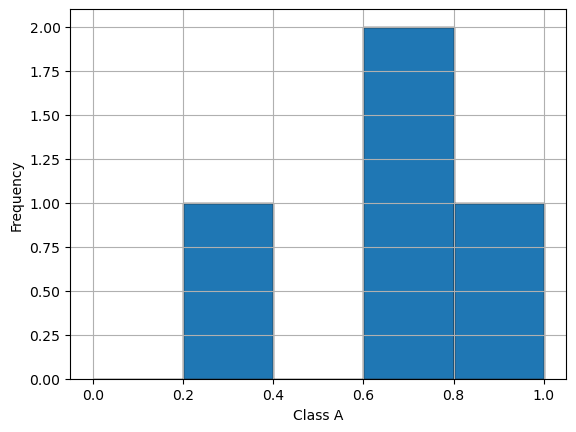
\includegraphics[width=.5\linewidth]{./assets/class_conditional_a.png}}\hfill
        \subfloat[]{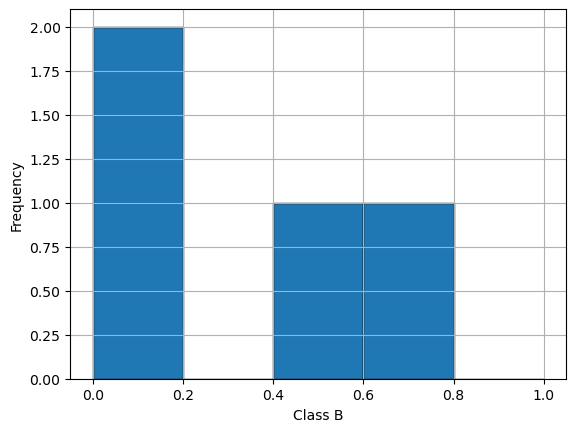
\includegraphics[width=.5\linewidth]{./assets/class_conditional_b.png}}\par
        \subfloat[]{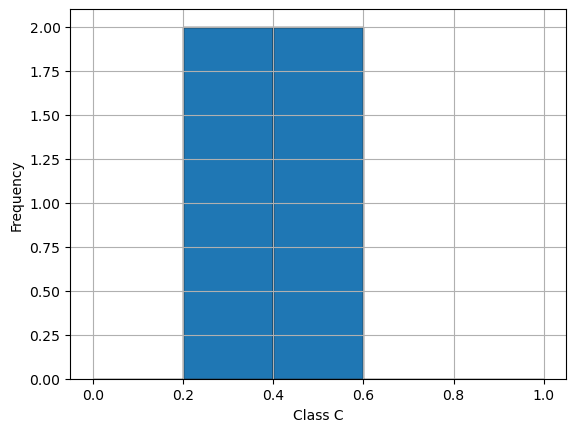
\includegraphics[width=.5\linewidth]{./assets/class_conditional_c.png}}
        \caption{Class-conditional relative histograms of $y_1$ with 5 equally spaced bins in $[0,1]$}
        \label{fig:class-conditional-y1}
    \end{figure}

    In order to find the root split using the discriminant rules from the empirical distributions, we made a decision tree with only a root split on $y_1$.
    Each branch will have the values of one bin, meaning there will be 5 branches (e.g. the first branch is for values of $y_1$ that belong to $[0,0.2[$).
    The leaf for each branch corresponds to the class that has the highest value for that specific bin in its histogram.

    \begin{figure}[H]
        \centering
        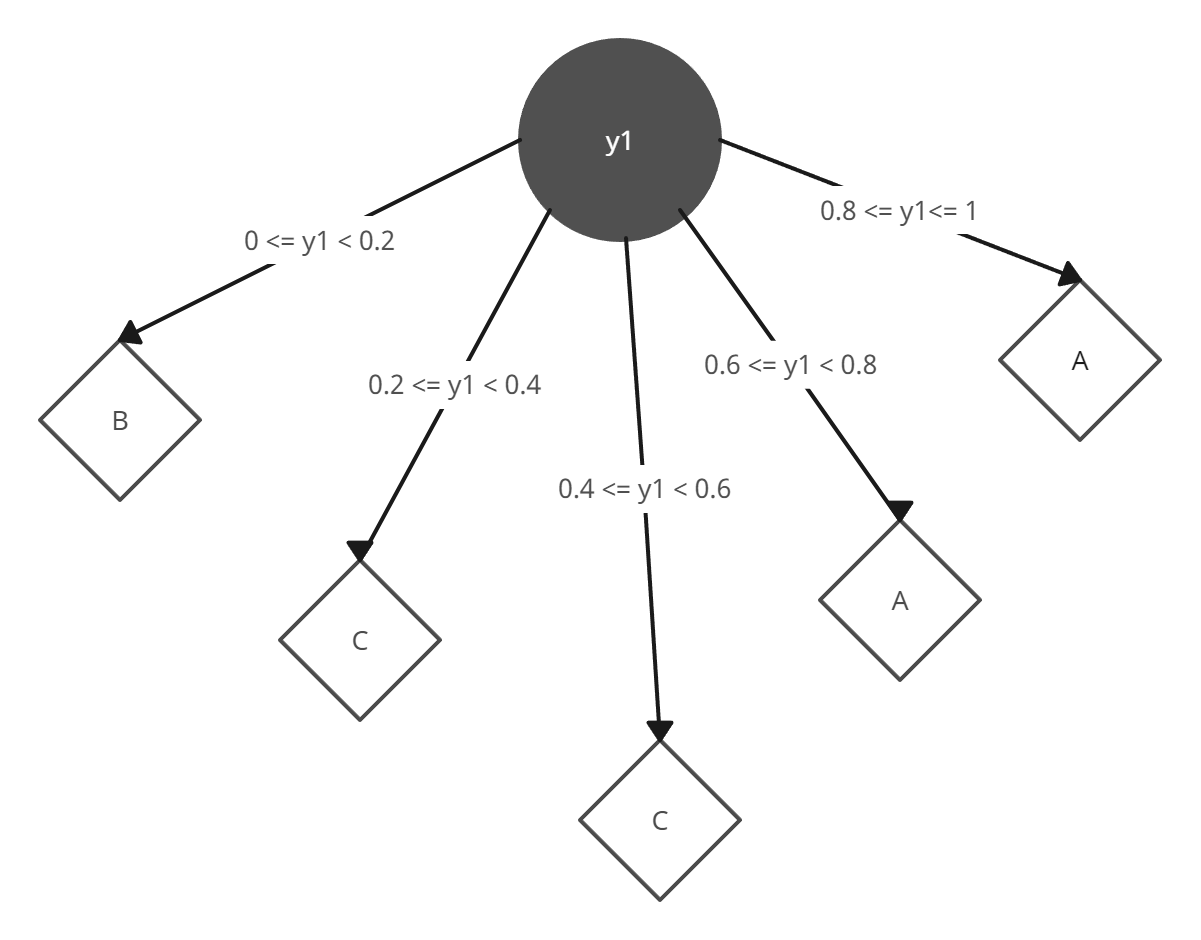
\includegraphics[width=12cm]{./assets/decision_tree_ex5_PartI.png}
        \caption{Decision Tree using the discriminant rules from the empirical distributions}
        \label{fig:decision-tree-root-split}
    \end{figure}

\end{enumerate}

\vskip 0.5cm

\begin{center}
\large{\textbf{Part II}: Programming}\normalsize
\end{center}

\noindent Consider the \texttt{column\_diagnosis.arff} data available at the homework tab, comprising 6 biomechanical
features to classify 310 orthopaedic patients into 3 classes (\texttt{normal}, \texttt{disk hernia}, \texttt{spondilolysthesis}).

\begin{enumerate}[leftmargin=\labelsep]
    \item \textbf{Apply \texttt{f\_classif} from \texttt{sklearn} to assess the discriminative power of the input variables.
          Identify the input variable with the highest and lowest discriminative power.
          Plot the class-conditional probability density functions of these two input variables.}

          \vskip 0.3cm
          \lstinputlisting[language=Python]{./assets/code_1.py}

          As you can see in the graph ahead, the highest discriminative power variable is \textit{degree\_spondilolysthesis} and
          the lowest discriminative power variable is \textit{pelvic\_radius}.

          \begin{figure}[H]
              \centering
              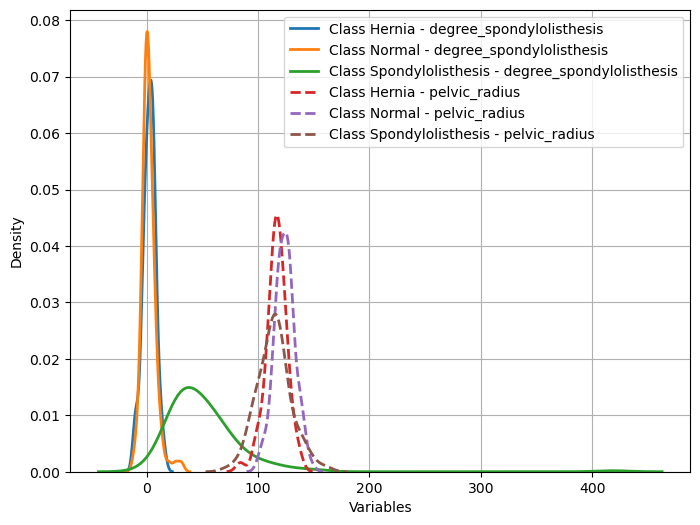
\includegraphics[width=12cm]{./assets/class_conditional_probability.png}
              \caption{Class-conditional probability density functions of the highest and lowest discriminative power variables.}
              \label{fig:PartII-ex1-plot}
          \end{figure}

    \item \textbf{Using a stratified 70-30 training-testing split with a fixed seed (\texttt{random\_state=0}), assess in a
          single plot both the training and testing accuracies of a decision tree with depth limits in
          $\{1,2,3,4,5,6,8,10\}$ and the remaining parameters as default.\vskip 0.05cm
          \textit{[Optional]} Note that split thresholding of numeric variables in decision trees is non-deterministic
          in sklearn, hence you may opt to average the results using 10 runs per parameterization.}

          \vskip 0.3cm
          \lstinputlisting[language=Python]{./assets/code_2.py}

          \begin{figure}[H]
              \centering
              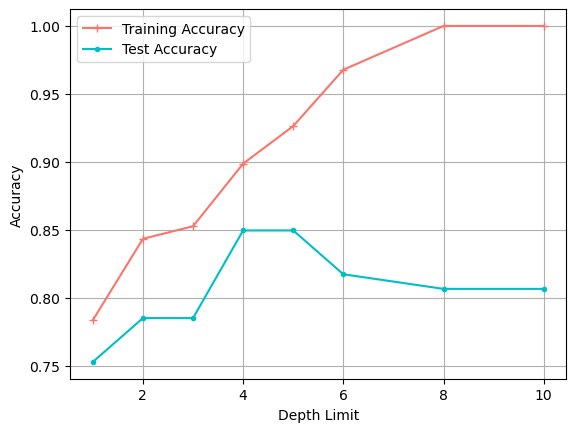
\includegraphics[width=12cm]{./assets/training_testing_accuracies.png}
              \caption{Accuracy of the trained decision tree, applied to both a test and training sets, for varying depth limits.}
              \label{fig:PartII-ex2-plot}
          \end{figure}

    \item \textbf{Comment on the results, including the generalization capacity across settings.}

          \vskip 0.3cm
          % Depth Limit and Training Accuracy
          The graphic shows that as the depth limit of the decision tree increases, the training accuracy rises steadily until reaching 100\%.
          This observation suggests that deeper trees can better fit the training data, capturing complex patterns and achieving higher accuracy when evaluated
          on the dataset.

          % Generalization Capacity
          The testing accuracy initially improves as the depth limit increases, indicating improved generalization. However, beyond a certain
          depth limit (around 4 or 5 in this case), the testing accuracy starts to decline. Therefore, we conclude there is a loss in generalization capacity,
          which causes overfitting, implying that, in this case, overly complex decision trees can fit noise in the training data, performing poorly on new, unseen data.

          % Optimal Depth Limit
          The optimal depth limit appears to be around 4 or 5, which seems to be the point where the accuracy is maximized for the testing data, striking a balance
          between model complexity and generalization to new data, this way we can avoid both underfitting (too simple) and overfitting (too complex).
          \vskip 0.3cm

    \item \textbf{To deploy the predictor, a healthcare team opted to learn a single decision tree
          (\texttt{random\_state=0}) using \textit{all} available data as training data, and further ensuring that each leaf has
          a minimum of 20 individuals in order to avoid overfitting risks.}
          \begin{enumerate}
          \item \textbf{Plot the decision tree.}

          \vskip 0.3cm
          \lstinputlisting[language=Python]{./assets/code_4_a.py}

          \begin{figure}[H]
              \centering
              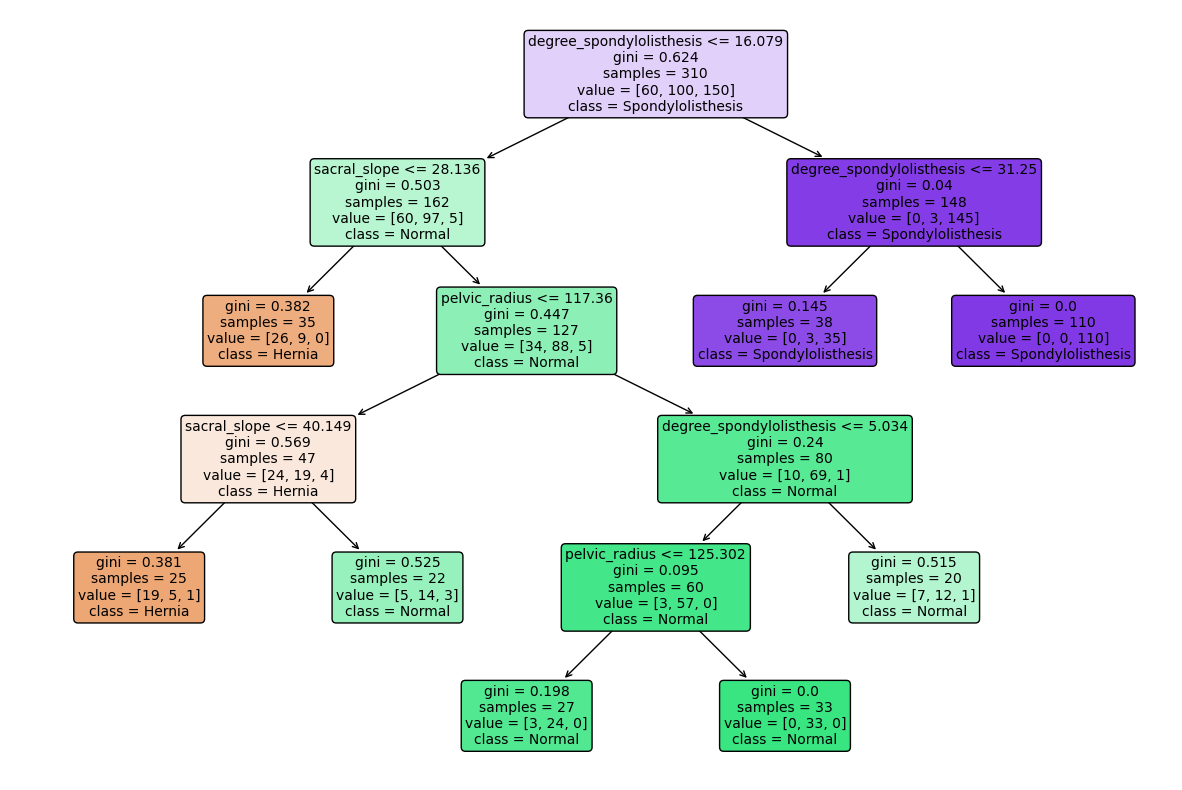
\includegraphics[width=\linewidth]{./assets/decision_tree_ex4a_PartII.png}
              \caption{Decision Tree for exercise II.4a}
              \label{fig:PartII-ex4a-plot}
          \end{figure}

          \item \textbf{Characterize a hernia condition by identifying the hernia-conditional associations.}

          \vskip 0.3cm

          The hernia condition can be characterized by:
          \begin{enumerate}
            \item degree\_spondilolysthesis $\leq 16.079$ and sacral\_slope $\leq 28.136$
            \item degree\_spondilolysthesis $\leq 16.079$, sacral\_slope $> 28.136$, pelvic\_radius $\leq 117.36$ and sacral\_slope $\leq 40.149$
          \end{enumerate}
          \end{enumerate}
\end{enumerate}

\end{document}
